\documentclass[a4paper,12pt,fleqn,twoside,openright]{memoir} 	% Openright aabner kapitler paa hoejresider (openany begge)

%%%% PAKKER %%%%

% ¤¤ Oversaettelse og tegnsaetning ¤¤ %
\usepackage[utf8]{inputenc}					% Input-indkodning af tegnsaet (UTF8)
\usepackage[danish]{babel}					% Dokumentets sprog
\usepackage[T1]{fontenc}					% Output-indkodning af tegnsaet (T1)
\usepackage{ragged2e,anyfontsize}			% Justering af elementer
% \usepackage{fixltx2e}						% Retter forskellige fejl i LaTeX-kernen (compileren siger dog at fixltx2e ikke længere er nødvendig)

																			
% ¤¤ Figurer og tabeller (floats) ¤¤ %
\usepackage{graphicx} 						% Haandtering af eksterne billeder (JPG, PNG, PDF)
\usepackage{multirow}                		% Fletning af raekker og kolonner (\multicolumn og \multirow)
\usepackage{colortbl} 						% Farver i tabeller (fx \columncolor, \rowcolor og \cellcolor)
\usepackage[dvipsnames]{xcolor}				% Definer farver med \definecolor. Se mere: http://en.wikibooks.org/wiki/LaTeX/Colors
\usepackage{flafter}						% Soerger for at floats ikke optraeder i teksten foer deres reference
\let\newfloat\relax 						% Justering mellem float-pakken og memoir
\usepackage{float}							% Muliggoer eksakt placering af floats, f.eks. \begin{figure}[H]
%\usepackage{eso-pic}						% Tilfoej billedekommandoer paa hver side
%\usepackage{wrapfig}						% Indsaettelse af figurer omsvoebt af tekst. \begin{wrapfigure}{Placering}{Stoerrelse}
%\usepackage{multicol}         	        	% Muliggoer tekst i spalter
%\usepackage{rotating}						% Rotation af tekst med \begin{sideways}...\end{sideways}

% ¤¤ Matematik mm. ¤¤
\usepackage{amsmath,amssymb,stmaryrd} 		% Avancerede matematik-udvidelser
\usepackage{mathtools}						% Andre matematik- og tegnudvidelser
\usepackage{textcomp}                 		% Symbol-udvidelser (f.eks. promille-tegn med \textperthousand )
\usepackage{siunitx}						% Flot og konsistent praesentation af tal og enheder med \si{enhed} og \SI{tal}{enhed}
\sisetup{output-decimal-marker = {,}}		% Opsaetning af \SI og decimalseparator
\usepackage[version=3]{mhchem} 				% Kemi-pakke til flot og let notation af formler, f.eks. \ce{Fe2O3}
%\usepackage{rsphrase}						% Kemi-pakke til RS-saetninger, f.eks. \rsphrase{R1}
\usepackage{upgreek}

% ¤¤ Referencer og kilder ¤¤ %
\usepackage[danish]{varioref}				% Muliggoer bl.a. krydshenvisninger med sidetal (\vref)
\usepackage{natbib}							% Udvidelse med naturvidenskabelige citationsmodeller
%\usepackage{xr}							% Referencer til eksternt dokument med \externaldocument{<NAVN>}
%\usepackage{glossaries}					% Terminologi- eller symbolliste (se mere i Daleifs Latex-bog)

% ¤¤ Misc. ¤¤ %
\usepackage{listings}						% Placer kildekode i dokumentet med \begin{lstlisting}...\end{lstlisting}
\usepackage{lipsum}							% Dummy text \lipsum[..]
\usepackage[shortlabels]{enumitem}			% Muliggoer enkelt konfiguration af lister
\usepackage{pdfpages}						% Goer det muligt at inkludere pdf-dokumenter med kommandoen \includepdf[pages={x-y}]{fil.pdf}	
\pdfoptionpdfminorversion=6					% Muliggoer inkludering af pdf dokumenter, af version 1.6 og hoejere
\pretolerance=2500 							% Justering af afstand mellem ord (hoejt tal, mindre orddeling og mere luft mellem ord)
\usepackage{pdfpages}


% Kommentarer og rettelser med \fxnote. Med 'final' i stedet for 'draft' udloeser hver note en error i den faerdige rapport.
\usepackage[footnote,draft,danish,silent,nomargin]{fixme}		


%%%% BRUGERDEFINEREDE INDSTILLINGER %%%%

% ¤¤ Marginer ¤¤ %
\setlrmarginsandblock{3.5cm}{2.5cm}{*}		% \setlrmarginsandblock{Indbinding}{Kant}{Ratio}
\setulmarginsandblock{2.5cm}{3.0cm}{*}		% \setulmarginsandblock{Top}{Bund}{Ratio}
\checkandfixthelayout 						% Oversaetter vaerdier til brug for andre pakker

%	¤¤ Afsnitsformatering ¤¤ %
\setlength{\parindent}{0mm}           		% Stoerrelse af indryk
\setlength{\parskip}{3mm}          			% Afstand mellem afsnit ved brug af double Enter
\linespread{1,1}							% Linie afstand

% ¤¤ Litteraturlisten ¤¤ %
\bibpunct[,]{[}{]}{;}{a}{,}{,} 				% Definerer de 6 parametre ved Harvard henvisning (bl.a. parantestype og seperatortegn)
\bibliographystyle{bibtex/harvard}			% Udseende af litteraturlisten.

% ¤¤ Dybde af overskrifter ¤¤ %
\setsecnumdepth{subsection}		 			% Dybden af nummerede overkrifter (part/chapter/section/subsection)
\settocdepth{subsection} 					% Dybden af overskrifter vist i indholdsfortegnelsen

% ¤¤ Lister ¤¤ %
\setlist{
  topsep=0pt,								% Vertikal afstand mellem tekst og listen
  itemsep=-1ex,								% Vertikal afstand mellem items
} 

% ¤¤ Visuelle referencer ¤¤ %
\usepackage[colorlinks]{hyperref}			% Danner klikbare referencer (hyperlinks) i dokumentet.
\hypersetup{colorlinks = true,				% Opsaetning af farvede hyperlinks (interne links, citeringer og URL)
    linkcolor = black,
    citecolor = black,
    urlcolor = black
}

% ¤¤ Opsaetning af figur- og tabeltekst ¤¤ %
\captionnamefont{\small\bfseries\itshape}	% Opsaetning af tekstdelen ('Figur' eller 'Tabel')
\captiontitlefont{\small}					% Opsaetning af nummerering
\captiondelim{. }							% Seperator mellem nummerering og figurtekst
\hangcaption								% Venstrejusterer flere-liniers figurtekst under hinanden
\captionwidth{\linewidth}					% Bredden af figurteksten
\setlength{\belowcaptionskip}{0pt}			% Afstand under figurteksten
		
% ¤¤ Opsaetning af listings ¤¤ %
\definecolor{commentGreen}{RGB}{34,139,24}
\definecolor{stringPurple}{RGB}{208,76,239}

\lstset{language=Matlab,					% Sprog
	basicstyle=\ttfamily\scriptsize,		% Opsaetning af teksten
	keywords={for,if,while,else,elseif,		% Noegleord at fremhaeve
			  end,break,return,case,
			  switch,function},
	keywordstyle=\color{blue},				% Opsaetning af noegleord
	commentstyle=\color{commentGreen},		% Opsaetning af kommentarer
	stringstyle=\color{stringPurple},		% Opsaetning af strenge
	showstringspaces=false,					% Mellemrum i strenge enten vist eller blanke
	numbers=left, numberstyle=\tiny,		% Linjenumre
	extendedchars=true, 					% Tillader specielle karakterer
	columns=flexible,						% Kolonnejustering
	breaklines, breakatwhitespace=true,		% Bryd lange linjer
}

% ¤¤ Navngivning ¤¤ %
\addto\captionsdanish{
	\renewcommand\appendixname{Appendiks}
	\renewcommand\contentsname{Indholdsfortegnelse}	
	\renewcommand\appendixpagename{Appendiks}
	\renewcommand\appendixtocname{Appendiks}
	\renewcommand\cftchaptername{\chaptername~}				% Skriver "Kapitel" foran kapitlerne i indholdsfortegnelsen
	\renewcommand\cftappendixname{\appendixname~}			% Skriver "Appendiks" foran appendiks i indholdsfortegnelsen
}

% ¤¤ Kapiteludssende ¤¤ %
\definecolor{numbercolor}{gray}{0.7}		% Definerer en farve til brug til kapiteludseende
\newif\ifchapternonum

\makechapterstyle{jenor}{					% Definerer kapiteludseende frem til ...
  \renewcommand\beforechapskip{0pt}
  \renewcommand\printchaptername{}
  \renewcommand\printchapternum{}
  \renewcommand\printchapternonum{\chapternonumtrue}
  \renewcommand\chaptitlefont{\fontfamily{pbk}\fontseries{db}\fontshape{n}\fontsize{25}{35}\selectfont\raggedleft}
  \renewcommand\chapnumfont{\fontfamily{pbk}\fontseries{m}\fontshape{n}\fontsize{1in}{0in}\selectfont\color{numbercolor}}
  \renewcommand\printchaptertitle[1]{%
    \noindent
    \ifchapternonum
    \begin{tabularx}{\textwidth}{X}
    {\let\\\newline\chaptitlefont ##1\par} 
    \end{tabularx}
    \par\vskip-2.5mm\hrule
    \else
    \begin{tabularx}{\textwidth}{Xl}
    {\parbox[b]{\linewidth}{\chaptitlefont ##1}} & \raisebox{-15pt}{\chapnumfont \thechapter}
    \end{tabularx}
    \par\vskip2mm\hrule
    \fi
  }
}											% ... her

\chapterstyle{jenor}						% Valg af kapiteludseende - Google 'memoir chapter styles' for alternativer

% ¤¤ Sidehoved/sidefod ¤¤ %

\makepagestyle{Uni}							% Definerer sidehoved og sidefod udseende frem til ...
\makepsmarks{Uni}{%
	\createmark{chapter}{left}{shownumber}{}{. \ }
	\createmark{section}{right}{shownumber}{}{. \ }
	\createplainmark{toc}{both}{\contentsname}
	\createplainmark{lof}{both}{\listfigurename}
	\createplainmark{lot}{both}{\listtablename}
	\createplainmark{bib}{both}{\bibname}
	\createplainmark{index}{both}{\indexname}
	\createplainmark{glossary}{both}{\glossaryname}
}
\nouppercaseheads											% Ingen Caps oenskes

\makeevenhead{Uni}{}{}{\leftmark}				% Lige siders sidehoved (\makeevenhead{Navn}{Venstre}{Center}{Hoejre})
\makeoddhead{Uni}{\rightmark}{}{}			% Ulige siders sidehoved (\makeoddhead{Navn}{Venstre}{Center}{Hoejre})
\makeevenfoot{Uni}{\thepage}{}{}							% Lige siders sidefod (\makeevenfoot{Navn}{Venstre}{Center}{Hoejre})
\makeoddfoot{Uni}{}{}{\thepage}								% Ulige siders sidefod (\makeoddfoot{Navn}{Venstre}{Center}{Hoejre})
\makeheadrule{Uni}{\textwidth}{0.5pt}						% Tilfoejer en streg under sidehovedets indhold
\makefootrule{Uni}{\textwidth}{0.5pt}{1mm}					% Tilfoejer en streg under sidefodens indhold

\copypagestyle{Unichap}{Uni}								% Sidehoved defineres som blank på kapitelsider
\makeoddhead{Unichap}{}{}{}
\makeevenhead{Unichap}{}{}{}
\makeheadrule{Unichap}{\textwidth}{0pt}
\aliaspagestyle{chapter}{Unichap}							% Den ny style vaelges til at gaelde for chapters
															% ... her
															
\pagestyle{Uni}												% Valg af sidehoved og sidefod (benyt "plain" for ingen sidehoved/fod)


%%%% EGNE KOMMANDOER %%%%

% ¤¤ Billede hack ¤¤ %										% Indsaet figurer nemt med \figur{Stoerrelse}{Fil}{Figurtekst}{Label}
\newcommand{\figur}[4]{
		\begin{figure}[H] \centering
			\includegraphics[width=#1\textwidth]{billeder/#2}
			\caption{#3}
			\label{#4}
		\end{figure} 
}

% ¤¤ Specielle tegn ¤¤ %
\newcommand{\decC}{^{\circ}\text{C}}
\newcommand{\dec}{^{\circ}}
\newcommand{\m}{\cdot}


%%%% ORDDELING %%%%

\hyphenation{In-te-res-se e-le-ment}											% Preamble indlaeses
\raggedbottom													% Soerger for at LaTeX ikke "straekker" teksten

%\includeonly{file1,file2}										% Inkluder kun specifikke filer (kommasepareret liste)

\begin{document}												% Starter dokumentet - obligatorisk


\frontmatter													% Forindhold - nummereres med romertal

%
	\begin{center}
	
		
		\begin{figure}
			\centering
			\includegraphics[width=0.7\linewidth]{C:/Users/Martin/Desktop/heatsink1}
			
			
		\end{figure}
		\vspace*{1cm}
		
			\vspace*{1cm}
		
		\textbf{Kølegitter}
		
		\textbf{Martin Knudsen}
		
		\vfill
		
		En undersøgelse af strømning, type og køleeffekt. 
		
		\vspace{2.0cm}
	\end{center}











\cleardoublepage												% Indsaetter tom side, saa naeste kapitel starter paa hoejre side (hvis noedvendigt)
%\include{formalia/titelblad}
\cleardoublepage
%\include{formalia/forord}
\cleardoublepage

%%%% Indholdsfortegnelse (TOC) %%%%

\phantomsection													% Kunstigt afsnit, som hyperlinks kan 'holde fast i'
\pdfbookmark[0]{Indholdsfortegnelse}{indhold}					% Tildeler en klikbar bookmark til den endelige PDF
\tableofcontents*												% Indholdsfortegnelsen (kaldet ToC) 

%\addtocontents{toc}{\protect\newpage}							% Fremtvinger sideskift i ToC hvis noedvendig (der hvor koden placeres)


\mainmatter														% Hovedindhold - nummereres fra side 1

%%%% Rapportindhold %%%% 										% Rapportindholdet boer IKKE indeholde broedtekst - KUN includede filer!

%% Indledende %%												% Opdel evt. i passende afsnit for overblikkets skyld

\section{Indledning}

Det termodynamiske system vi har valgt at skrive om til den skrevne projekt i thermodynamik er i overordnede træk luftdrevne processor-kølere. 
Da forfatterne personligt interesserer sig for opbygning af PC, herunder køling som er en meget vigtig faktor.
Computere med dertilhørende køling og termodynamiske systemer fylder meget i hverdagen, men vi ved meget lidt om d termodynamiske processer i en PC.
Herunder kølere brugt i såvel kerne processorerne(CPU) som de grafiske processorer(GPU). For en god ordens skyld, har vi valgt at sige at systemgrænserne går imellem processoren og det køletekniske system, således at processoren og dets interface med det køletekniske system er adskilt fra det termodynamiske system.
Processorerne kommer da til at definere energistrømmene ud af systemet og den varme der skal ud af systemet.

Lauritzens og Eriksen, Termodynamik danner grundlagt for beregninger i skrivelsen der følger samt tabel opslag for diverse værdier. 
\section{felt}

Der er 4 forskellige slags kølinger der vil blive undersøgt i denne rapport: 

\begin{itemize}
	\item kølegitre(Heatsink)
	\item Varmerør(heatpipes)
	\item blæser/fluid(el.andet flow)
	%\item og fasekølinger
\end{itemize}


der er et overraskende stort udvalg af kølesystemer til processorer, og alt for mange til at de alle kan blive nævnt eller behandlet udtømmende i denne rapport. Men fælles for dem alle, er at de på en eller anden vis har fysisk forbindelse til processoren.
Vi vil ikke forholde os til køling og luftgennemstrømning af det kabinet som processor og kølesystem befinder sig i. Ikke fordi, der ikke sker termodynamiske ting i det, men fordi det umiddelbart, uden dybdegående inspektion, mere drejer sig om bortledning af opvarmet luft end om bortledning af varme og måske ikke et direkte termodynamisk emne.

I denne rapport, vil vi undersøge og sammenligne effekten af de forskellige kølesystemer, når varmen afledes til sidsti kølesystemet, samt finde et udtryk for den effekt processoren kan afsætte i kølesystemet og forsøge at dimensionere et kølesystem til en PC.



%% Kontekst %%

\section{Beskrivelse}

Moderne CPU og GPU enheder er bygget op af millionvis af elektroniske transistorer.  Disse transistorer er konstruret af halvledermaterialer, som typisk kun bevarer deres halvlederegenskaber indenfor et bestemt temperaturområde. Bliver disse udsat for konstante drifttemperaturer udenfor dette område, degraderer ikke bare deres elektriske signaler (med nedsat stabilitet i form af regnefejl og signalfejl) men også selve halvleder materialet de er konstrueret af, med betydelig nedsættelse af levetiden til følge.

Forfatterne noterer sig at GPU enhederne i en moderne PC fylder mere og mere i trit med at udviklingen af software og skærme betyder at der skal foretages flere og flere beregninger.  Det betyder at der rent fysisk skal bruges flere transistorer og typisk mere energi i en GPU for at opnå det ønskede ydelsesniveau.

Det betyder reelt at termodynamik i allerhøjeste grad indgår i design, funktion og brug af en computer.

I kølesystemet for en computerprocessor foregår den første varmetransmission som varmeledning fra processorens varmespreder til kølesystemet.
Ofte faciliteres denne varmetransmissionen af en kølepasta, som er med til at maksimere kontaktfladen til kølesystemet og som modvirker galvanisk tæring.
I kildelisten er inkluderet to eksempler på kølepasta, med konduktivitets værdier på hhv. 0,8 og 12,5 W/m*K.
Intentionen med kølepasta er at optimere overflade kontakten imellem kølegitter og processor og undgå at der opstår små luftfyldte områder, hvor der kan dannes ekstra varmemodstand. Dog vil laget af kølepasta her blive betragtet som liggende udenfor systemgrænsen.

Det umiddelbare indtryk er dog at GPU og CPU i termodynamisk forstand er identiske, hvorfor ordet CPU vil brugt i flæng om både CPU og GPU.

Den elektriske effekt P afsat i en CPU kan beskrives således :

 P = strømforbrug (I) * taktfrekvens (f) * kapacitans (C) .

 (kilde :ftp://download.intel.com/design/network/papers/30117401.pdf)


\section{Processor}

Den elektriske effekt P afsat i en CPU kan beskrives således :

 P = strømforbrug (I) * taktfrekvens (f) * kapacitans (C) .

 (kilde: ftp://download.intel.com/design/network/papers/30117401.pdf)

I kølesystemet for en computerprocessor foregår den første varmetransmission som varmeledning fra processorens varmespreder til kølesystemet.

Ofte faciliteres denne varmetransmissionen af en kølepasta, som er med til at maksimere kontaktfladen til kølesystemet og som modvirker galvanisk tæring.

I kildelisten er inkluderet to eksempler på kølepasta, med konduktivitets værdier på hhv. 0,8 og 12,5 W/m*K.

Intentionen med kølepasta er at optimere kontakten mellem kølegitter og processor og undgå at der opstår små luftlommer, hvor der kan dannes ekstra varmemodstand. Dog vil laget af kølepasta her blive betragtet som liggende udenfor systemgrænsen.

De fleste kølegitre er lavet af aluminum, som har en varmekonduktivitet er på 229 W/m*K.

Vi antager et endimensionelt, stationært system med konstant varmestrøm. Vi antager ydermere konstant densitet og temperatur på den omgivende, tørre atmosfæriske luft.

FIXME:
Tykkelserne på godset i den retning varmen udbredes i er 0.5 mm for kølegitteret og regnes som en massiv væg, idet processoren regnes for at have en ens temperatur i hele sit areal.  Varmen forsimples til at udbredes i en retning og i et stationært system.  Med disse antagelser kan varmestrømmen igennem lamellerne beregnes.
Luften antageds at flytte sig 0.01 m/s


%% Teknisk %%
\section{Metode}

Der søges at udregne varmestrømmene for de forskellige komponenter, således at disse kan indgå i sammenligning af varme og temperatur.

\begin{enumerate}
	\item Klarlægning af flowgeometrien
	\item Beregn Referencetemperatur
	\item Bestem kendetal(Re, Gr, Ra, Pr)
	\item Vælg modelligning
	\item Beregn varmeovergangstallet ud fra Nusselts tal
\end{enumerate}

Det antages at processoren afgiver 100 \% af sin varme i kølesystemet.
Systemgrænserne udgøres (som tidligere nævnt) af interfacet til processoren og af bortledning af varme fra den sidste komponent i kølesystemet.
%Vi vil søge at sammenligne den effekt de respektive komponenter bortleder for at kunne sætte et udtryk op for hvor meget strøm Processoren kan afsætte.

FIXME: Her bør være en illustration set fra siden.
\begin{figure}
	\centering
	\includegraphics[width=0.7\linewidth]{"../../../../../../../one drive/OneDrive - Aarhus universitet/TD projekt/KF.png}
	\caption{kontrolflader for systemet der regnes på.}
	\label{fig:kf}
\end{figure}

\begin{figure}
	\centering
	\includegraphics[width=0.7\linewidth]{billeder/heatsink1}
	\caption{Eksempel på kølegitter, fra grabcad.com - bruger: Fernando}
	\label{fig:heatsink1}
\end{figure}


\begin{figure}
	\centering
	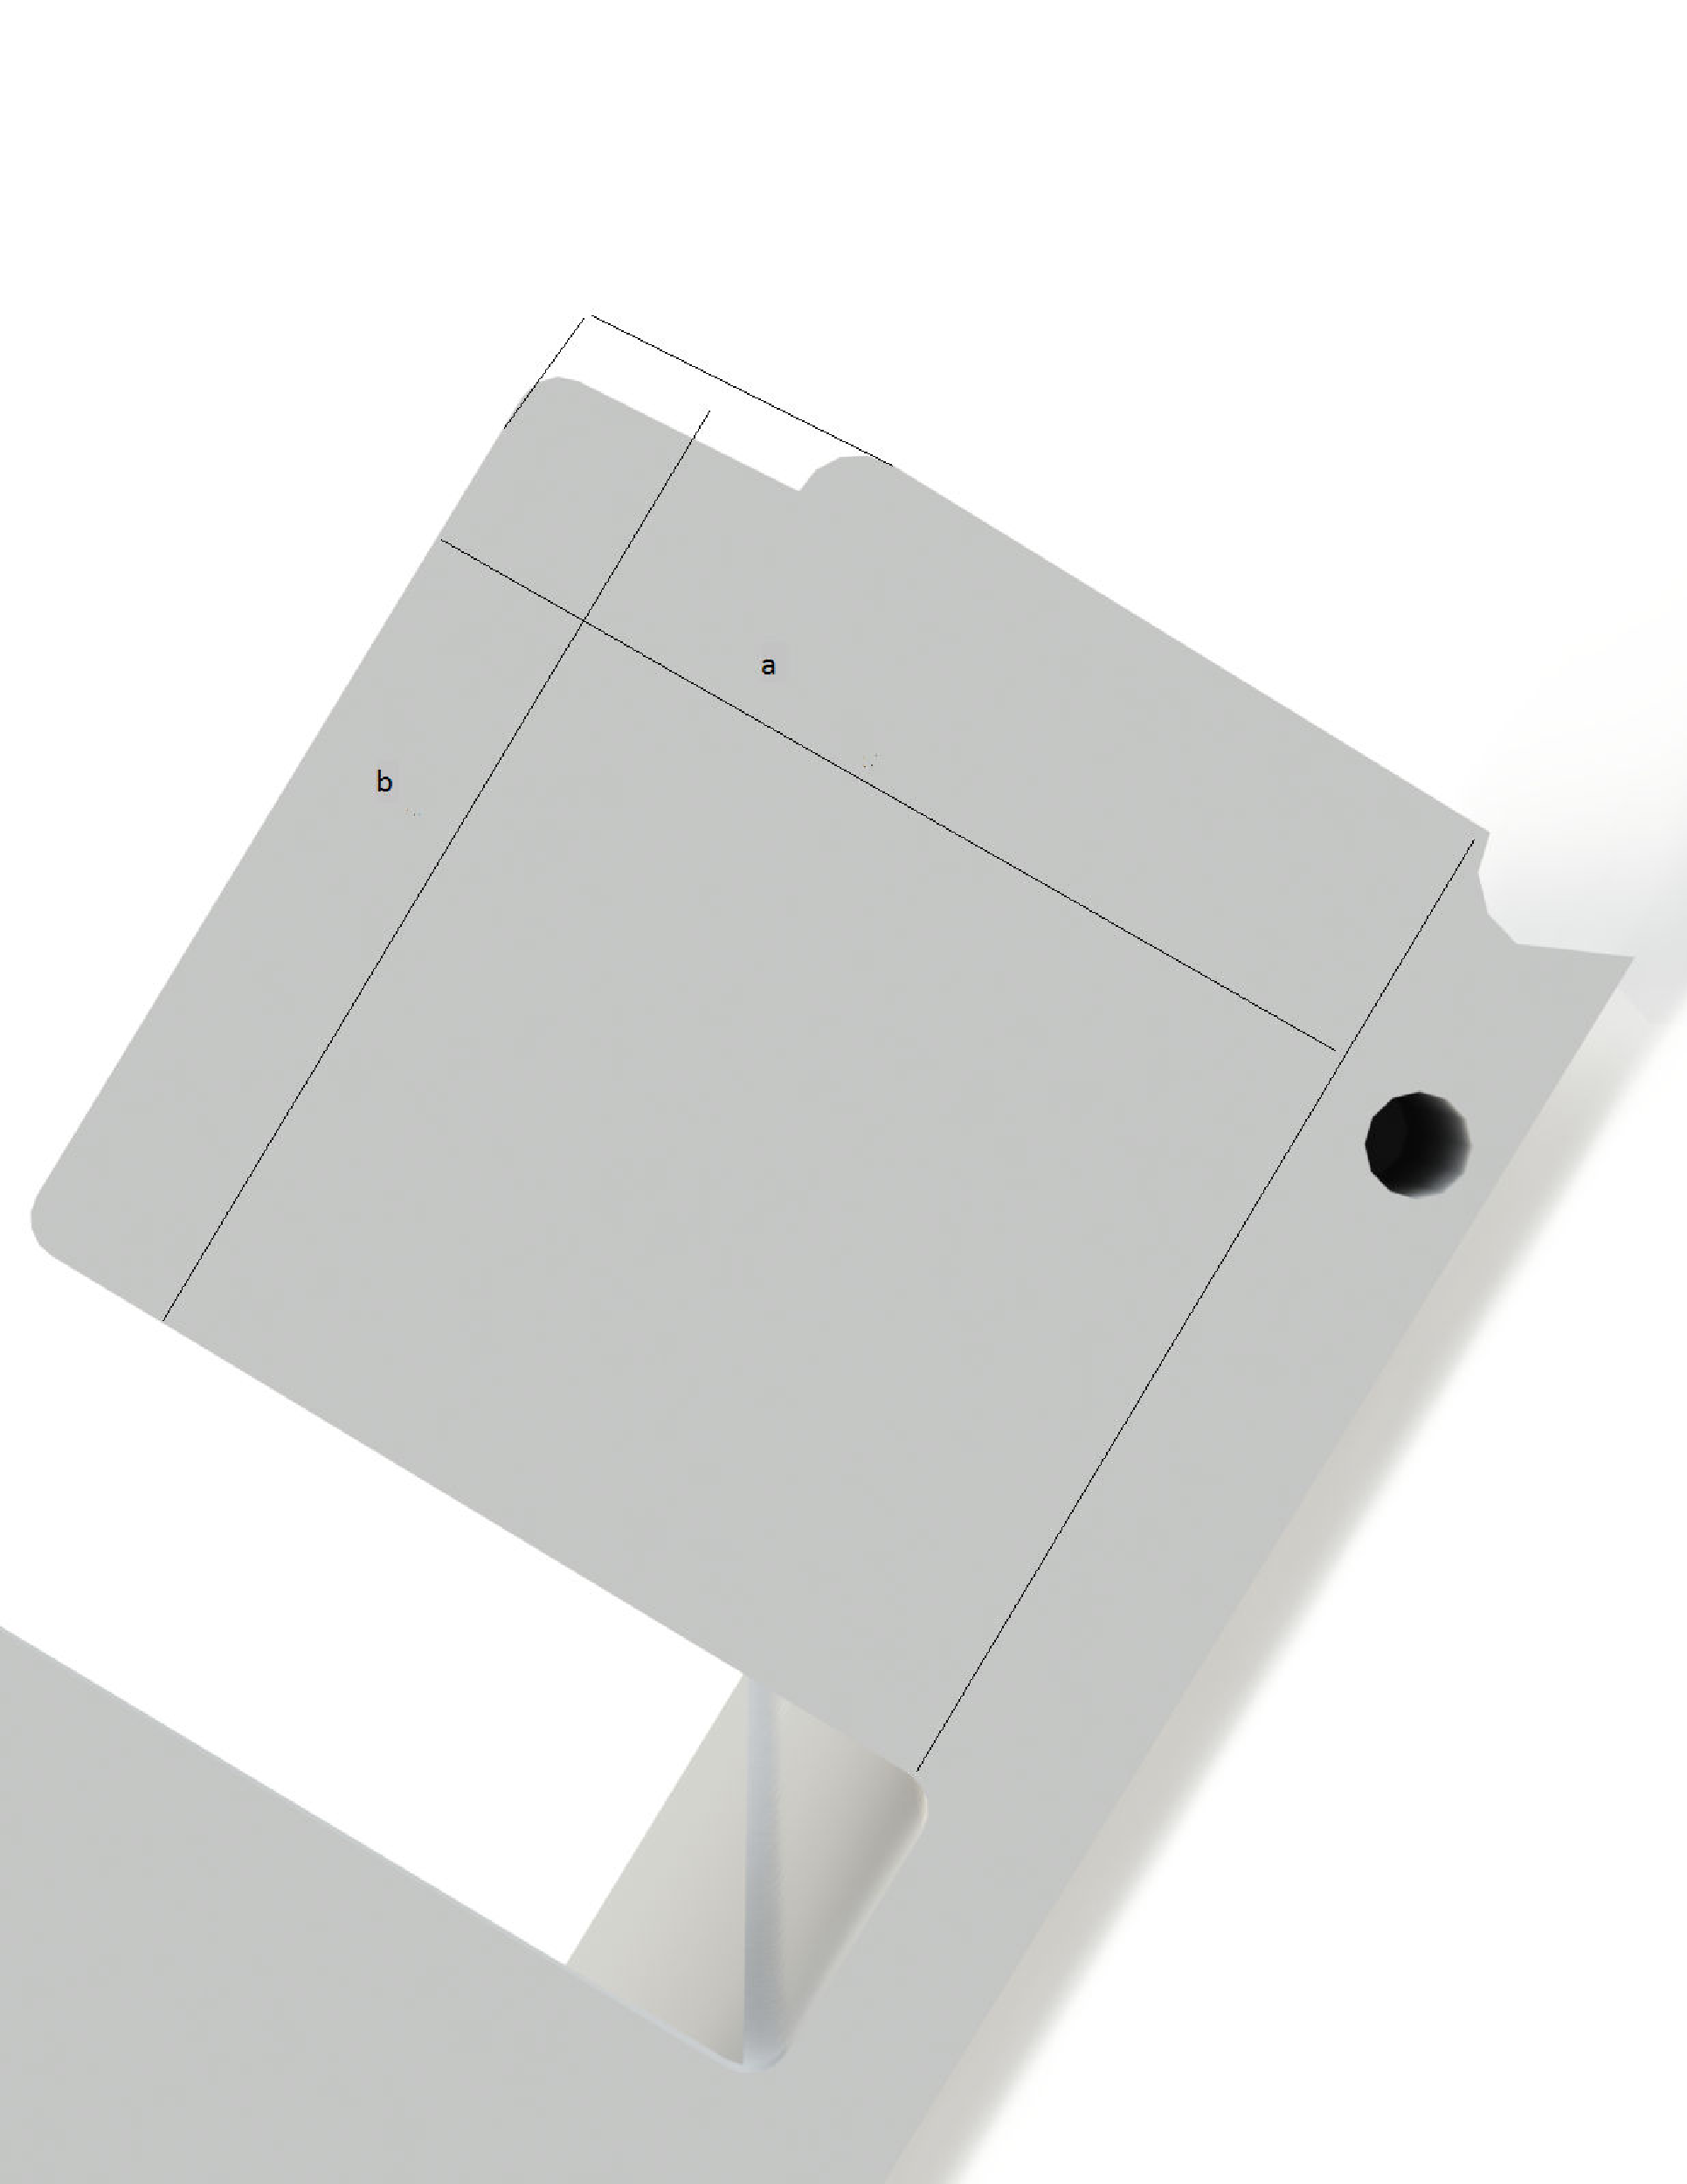
\includegraphics[width=0.7\linewidth]{billeder/lamel}
	\caption{Lamel. Genstand for vore termdynamiske undersøgelser. fra grabcad.com - bruger: Fernando}
	\label{fig:lamel}
\end{figure}
\section{Gitter}

Fælles for alle 3 systemer er kølegitteret af aluminium, der er i kontakt med processoren. 
I simple systemer udgør den den eneste part i kølesystemet og kan selvfølgelig bestå af andre materialer end Aluminium. 
Men i rapporten her vil aluminum blive brugt

Kølegitteret udnytter overfladeareal til at bortlede varme ved konvektion fra et fast materiale(aluminium) til et fluid(atmosfærisk luft) .
Således vil der være to termiske modstande, navnlig varmeledningsmodstand og varmeovergangsmodstand.

En hyppig forekommende struktur i et kølegitter er ribbe, der giver en naturlig strømning af den varme luft bort fra kølegitteret. Hvor kun er termodynamiske kræfter har indflyldelse på strømningen. Men strømningen foregår foregår imellem to kanalvægge. 

Der præsenteres her en oversigt over de værdier der bruges i udregningerne: 

Der beregnes varmestrøm for konvektion og for stråling.

Tallene for ovenstående kølegitter er importeret fra en partfil i Solidworks. %Kanalen for strømningen af luft der regnes for er d(1mm) bred og den hydraulisk diameter regnes som værende en snæver kanal, hvor L=2*a

H = 20 mm, $b = 25,5 mm$, $d  =1 mm$ ,Areal $A_t = 93733.73 mm^2$ , $A_{lam}= 500 mm^2$  \\ 
$ Massen m = 31,58 gr.$ \\
Varmekonduktiviten for aluminium, $\lambda_{al} = 228$ \\  
Lameltykkelsen $\delta = 0.5 mm.$  \\\
Den specifikke varmekapacitet $c\_p = 1.008$ \\
Strømningshastighed lodret, i lamellets længde på $c = 0.001$ \\



For at udregne varmestrømmen $\phi$  bruges udtrykket \\ $\Phi = \alpha * A* (t\_{fl}-t\_v$ \\  også kendt som Newtons ligning. \\ 
Hvoraf varmekonduktiviteten $\alpha$ er fundet ved tabel opslag $\alpha = 21.8$ \\
Kinematisk viskositet er: $18.88$ og dynamisk viskositet = $16.92$  \\
Volumenudvidelseskoefficienten $\beta_luft = 3,2$ \\
 
Varmeledningsmodstanden : $R_l = \frac{\delta}{\lambda_{al}*A_{lam}} = 4.281$ \\
Varmeovergangsmodstanden : $R_o = \frac{1}{\alpha_{tl}*A_{lam}} = 89.394$ \\

Total termisk modstand er $R_{tot} = R_l + R_o = 92.225$ \\

\section{Beregninger}

Varmestrømmen $\phi$ udregnes ved ligningen Nu = $\frac{\alpha}*{\lambda}$ \\
Nu er Nusselts tal og findes herunder ved at udregne Reynolds(Re) og Prandtls(pr) tal.


Strømningsforholdende for luft(fluiden) imellem lammelerne i gitteret er fri indvendig strømning, idet, lamellerne kan ses som kanalvægge og udgangen i en antaget lodret given retning er smal og bred. med 3 åbne sider og derved tillader en fri udvikling af strømningen. Hvor den dydrauliske diameter er i brug og sættes lig med afstanden imellem 2 givene lameller. $\approx 0.5 mm$

Reference temperaturen udregnes til : 
\\$t_{film} = \frac{{t_{lam}}+t_{fluid}}{2} => t_{film}=30$
\\Grasshofs tal Gr = $\frac{g*L^3*\beta*{\Delta\,t}}{\upsilon\,^2} = 8,771*10^4$
\\Prandtls tal Pl(opslag) => $Pr=0.69$


Der antages lodret  strømning af luften og Reynold tal undersøges for at få et hit om strømningsformen\\

$Re = \frac{c_{luft}*L_{hyd}}{\upsilon} = 2.648*10^{-5}$
%$ Ra = Gr*Pr = 6.052*10^4$ => \\ 
Hvilket indikerer laminar strømning over hele længden af et lamel. 
Hvorfor strømningen ikke undersøges yderligere, idet Re er $10^9$ mindre, end den forventede kritiske værdi for turbulent strømning.

Hastghedsprofilet hvorved den opvarmede luft stiger til vejr er udregnet til: 
$0.05*Re*L_{hd} = 0.001 $

Hvilket medfører at Nusselts tal kan udregnes som \\ 
$Nu = 3,66+ \frac{0.0668*Re*Pr*\frac{D}{L_{lam}}}{1+0.004*()\frac{D}{L_{lam}}k *Re*Pr})^{2/3} = 3.661$


%Den kritisk værdi findes da ved: $Nu_m = C*Ra^4$

og $ \Phi = \alpha*A(t_{fl}-t_v =>2.597*10^6 W $\\ 
justeret til milimeter ved udtrykket: $\frac{\Phi = \alpha*A*(t_{fl}-t_v}{10^6} =>0.75 W$

samtlige lammeler afgiver da $0,75 w* 40 \approx 30 W$ i varmestrøm til luften der passerer. 

\begin{figure}
	\centering
	\includegraphics[width=0.7\linewidth]{billeder/heatsink1}
	\caption{Eksempel på kølegitter, Fra grabcad.com - bruger: Fernando}
	\label{fig:heatsink1}
\end{figure}


\begin{figure}
	\centering
	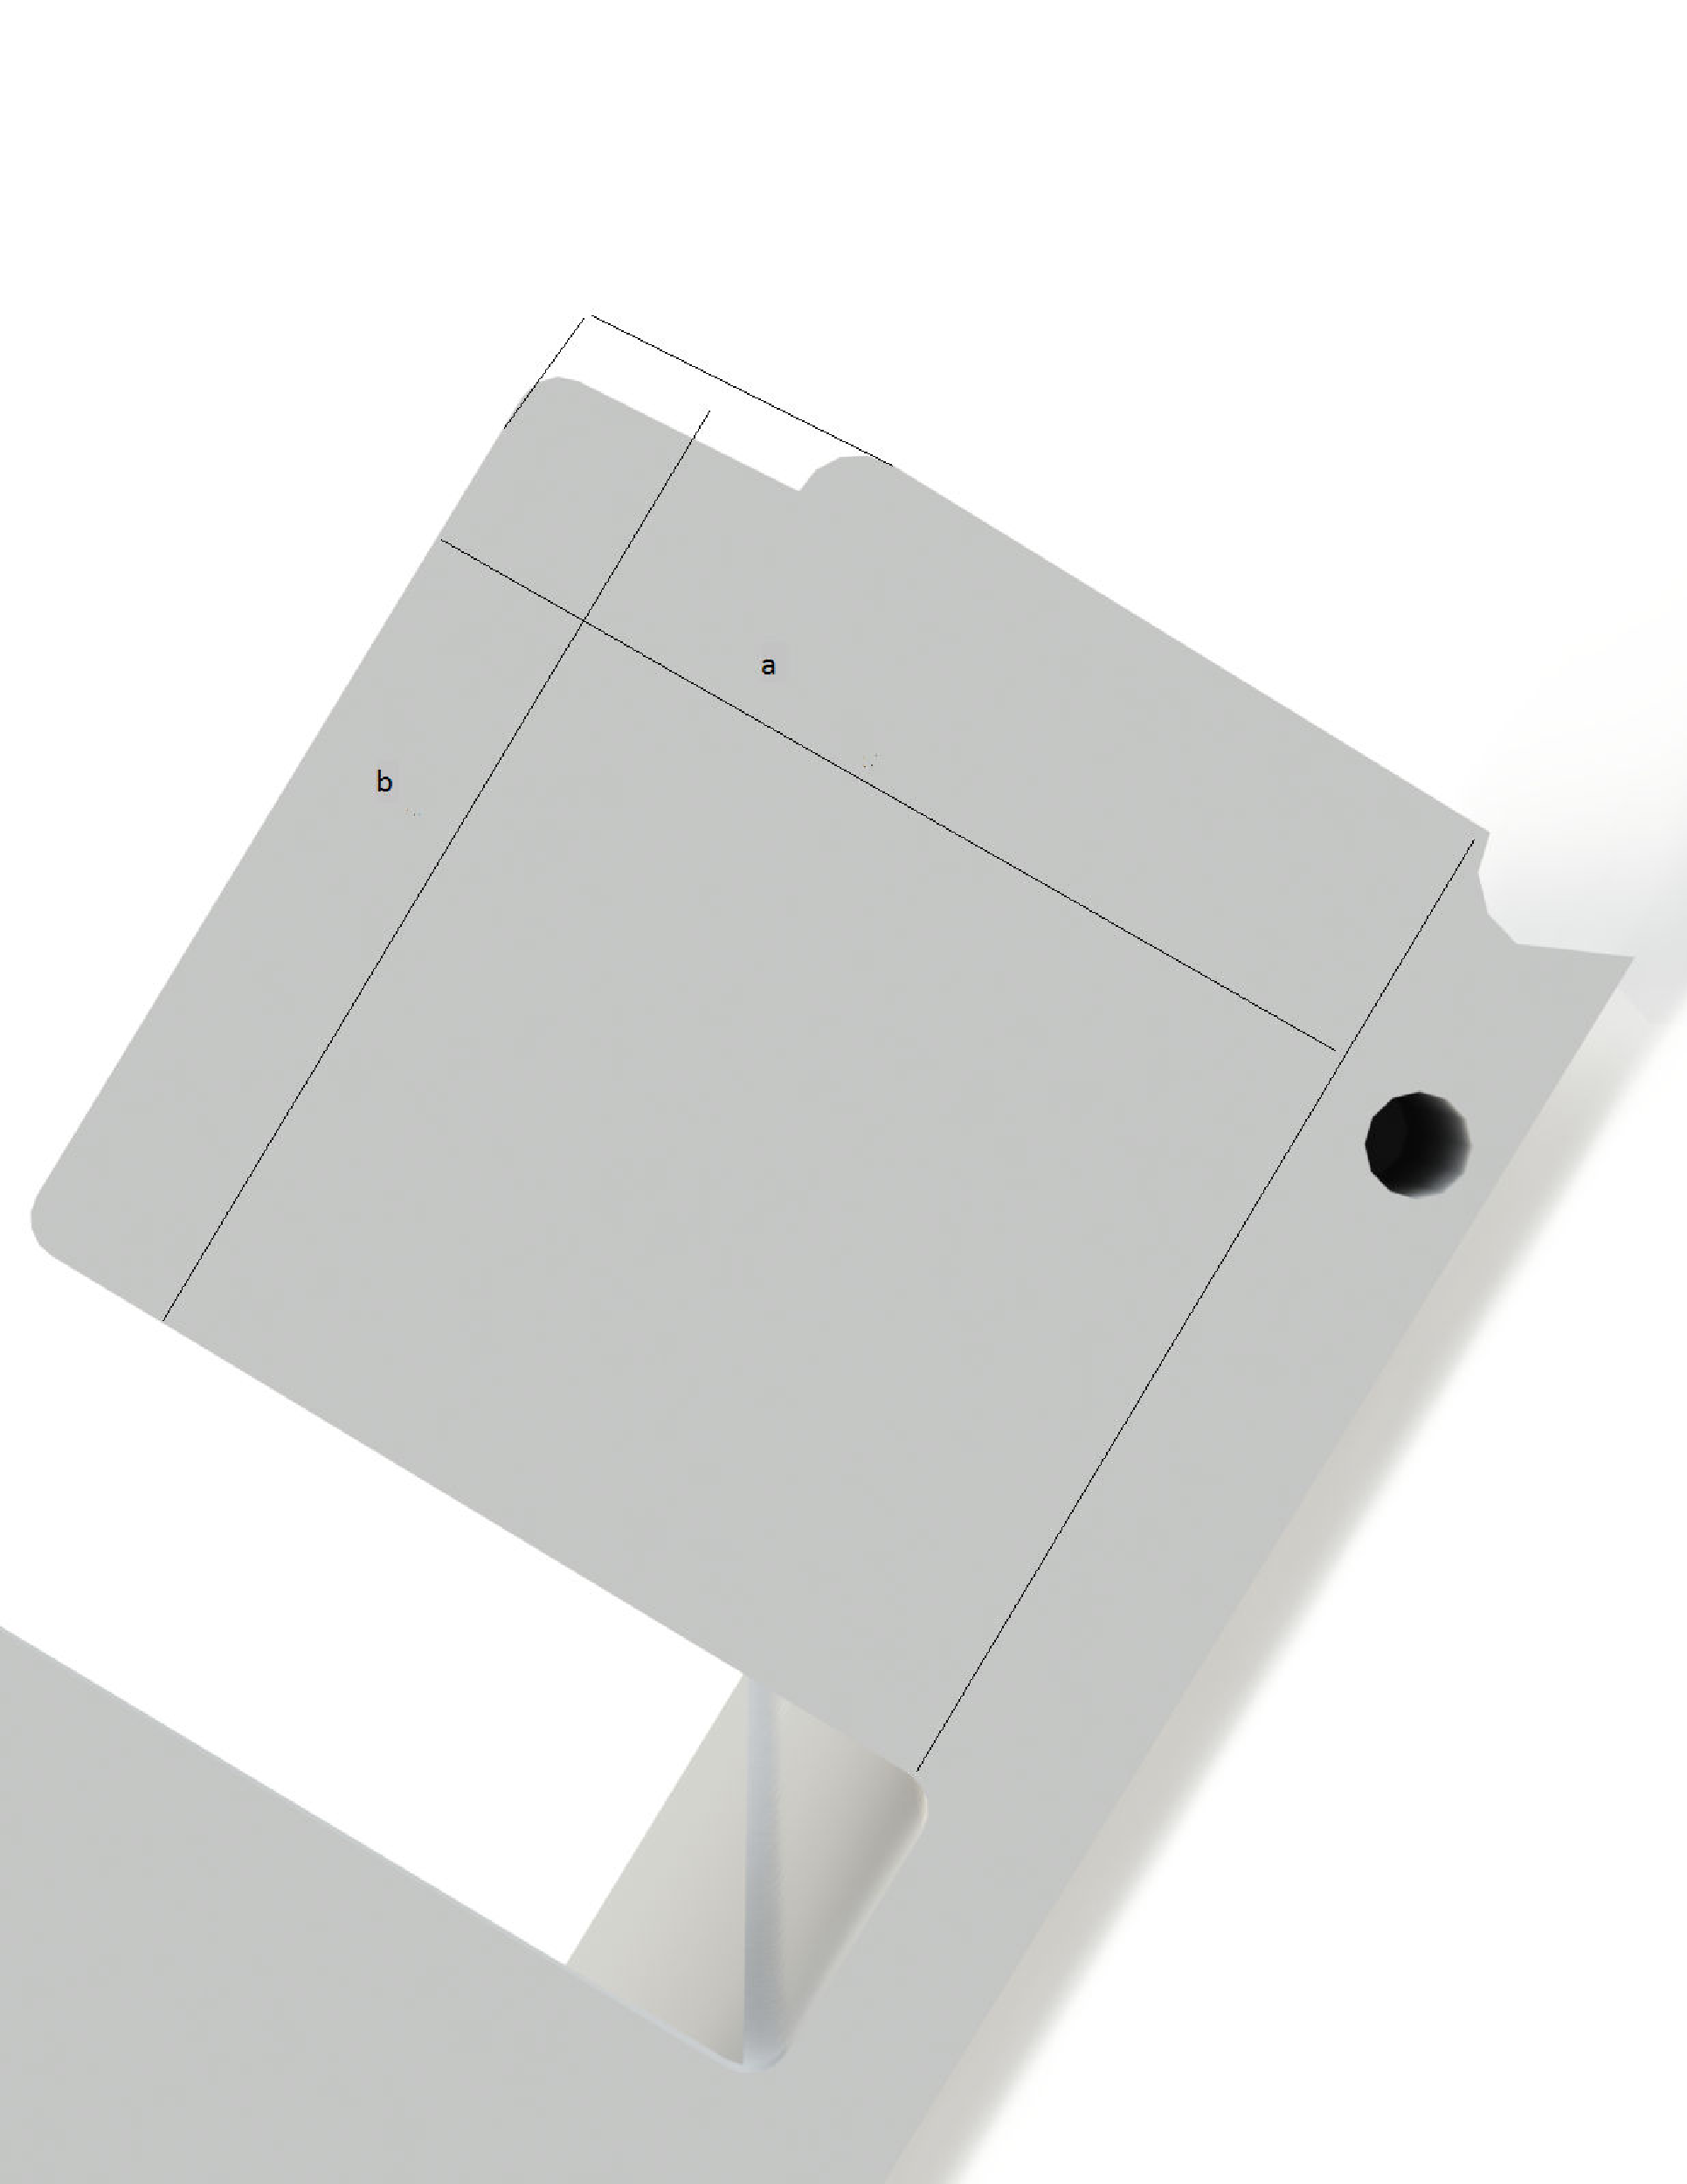
\includegraphics[width=0.7\linewidth]{billeder/lamel}
	\caption{Lamel. genstand for vore termdynamiske undersøgelser.Fra grabcad.com - bruger: Fernando}
	\label{fig:lamel}
\end{figure}

\section{Heatpipe}

For en varmeledende kobberrør, uden blæser installeret vil der bliver tilført en ekstra overflade hvorfra der kan foregå varmeovergang såvel som varmestråling.
Varmestrømmen.

Et sådan varmerør kan være opbygget på lidt varierende måde fra en hul rør med en rektaunglær profil indeholdende vædsker, til en solid profil. 

%% Afrunding %%

%\section{Konklusion}

Et varmegitter af aluminium forekommer umiddelbart at være en relativt effektiv måde at aflede varmen på. 
Den store hindring i varmetransmissionenforekommer at være overgangsmodstanden for luft. 
Materialet lader ikke til at gøre en synderlig forskel, dog skal det bemærkes at aluminium er et af de mest varmeledende materialer, billigt, let og nemt at forarbejde.

Ulempen ved sådan en konstruktion her er, at fluidets filmlag er relativt tykt og har laminart flow, hvorfor luftudskiftningen er lidt langsom og mindre effektiv i konvektion. 
Men materialet er generelt underordnet ift. laminart/turbulent flow og det samlede overfladeareal, hvorfor det giver god mening at aluminium bruges i vid udstrækning til pc kølesystemer. 


%%%% Kilder %%%%

\begingroup
	\raggedright
	\bibliography{bibtex/litteratur}							% Litteraturlisten inkluderes
\endgroup


%%%% Fixme-listen %%%%

\newpage														% Ny side til Fixme-listen
\listoffixmes													% Fixme-listen - fjernes til sidst i projektet med "%"


%%%% Appendiks %%%%

\appendix														% Appendiks/bilag start - giver chapter bogstaver i stedet for tal
\clearforchapter												% Sikrer at pagestylen aktiveres paa den rigtige side
\phantomsection													% Kunstigt afsnit, som hyperlinks kan 'holde fast i'
\pdfbookmark[0]{Appendiks}{appendiks}							% Tildeler en klikbar bookmark til den endelige PDF

%% Indstillinger for appendiks (deaktiveret med "%") %%

%\pagestyle{empty}												% Sidehoved/-fod for standardsider aendres til tom for appendiks
%\aliaspagestyle{chapter}{empty}								% Sidehoved/-fod for kapitelsider aendres til tom for appendiks
%\settocdepth{chapter}											% Kun kapitel-niveau vises i ToC
%\addtocontents{toc}{\protect\cftpagenumbersoff{chapter}}		% Sidetal for kapitler fjernes i ToC

%% Filer til appendiks %%

%\include{appendiks/appendiks1}


%%%% Bilag %%%%

%\phantomsection												% Kunstigt afsnit, som hyperlinks kan 'holde fast i'
%\addcontentsline{toc}{chapter}{Bilag A \ Navn} 				% Manuelle indgange i indholdsfortegnelsen (naar \includepdf bruges)

%\includepdf[pages={x-y}]{filnavn}								% Inkluder eksterne bilag med \includepdf[pages={x-y}]{filnavn}


\end{document}													% Slutter dokumentet - obligatorisk


